\documentclass[french,12pt]{report}

\usepackage[utf8]{inputenc}
\usepackage[T1]{fontenc}
\usepackage{babel}
\usepackage{setspace}
\usepackage{graphicx}
\usepackage{afterpage}
\usepackage[margin=3em]{geometry}
\usepackage{color}
\usepackage[svgnames]{xcolor}
\usepackage{textcomp}
\usepackage{listingsutf8}
\usepackage{pdfpages}
\usepackage[linkbordercolor=teal]{hyperref}
\usepackage{glossaries} %https://tex.stackexchange.com/questions/133269/how-to-update-glossaries-package-on-ubuntu-12-10#133544

%https://tex.stackexchange.com/questions/10141/how-to-prevent-lstlisting-from-splitting-code-between-pages#10145
\lstnewenvironment{Code}[1][]{
   \noindent
   \minipage{\linewidth}
   \vspace{0.5\baselineskip}
   \lstset{
   % https://stackoverflow.com/questions/586572/make-code-in-latex-look-nice
   % https://tex.stackexchange.com/questions/50107/adjust-bottom-margin-of-a-listing-environment#50108
   % https://en.wikibooks.org/wiki/LaTeX/Source_Code_Listings
     aboveskip=\bigskipamount,
     keywordstyle=\color{RoyalBlue},
     basicstyle=\scriptsize\ttfamily,
     commentstyle=\color{Green}\ttfamily,
     rulecolor=\color{black},
     upquote=true,
     numbers=left,
     numberstyle=\tiny\color{gray},
     stepnumber=1,
     numbersep=8pt,
     showstringspaces=false,
     breaklines=true,
     frameround=ftff,
     frame=single, %shadowbox
     inputencoding=utf8/latin1,
     language=Python,
     #1,
   }
}{\endminipage}

\parindent=2.2em
\parskip=.7em
\renewcommand{\FrenchLabelItem}{\textbullet}
\renewcommand{\UrlFont}{\ttfamily\scriptsize}
%\renewcommand{\glstextformat}[1]{\textcolor{blue}{#1}} % couleur des liens vers le glossaire

%https://tex.stackexchange.com/questions/63390/how-to-decrease-spacing-before-chapter-title#63393
\makeatletter
\def\@makechapterhead#1{%
  %%%%\vspace*{50\p@}% %%% removed!
  {\parindent \z@ \raggedright \normalfont
    \ifnum \c@secnumdepth >\m@ne
        \huge\bfseries \@chapapp\space \thechapter
        \par\nobreak
        \vskip 20\p@
    \fi
    \interlinepenalty\@M
    \Huge \bfseries #1\par\nobreak
    \vskip 40\p@
  }}
\def\@makeschapterhead#1{%
  %%%%%\vspace*{50\p@}% %%% removed!
  {\parindent \z@ \raggedright
    \normalfont
    \interlinepenalty\@M
    \Huge \bfseries  #1\par\nobreak
    \vskip 20\p@
  }}
\makeatother

\newcommand{\projectroot}{../../../..}
\newcommand{\srcroot}{\projectroot/src}
\newcommand{\srcpyroot}{\srcroot/python}
\newcommand{\srcresroot}{\srcroot/res}

\newcommand{\rapportroot}{\projectroot/documents/out/rendus/rapport}
\newcommand{\rapportresroot}{\rapportroot/res}
\graphicspath{{\rapportresroot/img/}}
\newcommand{\txtroot}{\rapportresroot/txt}

\newcommand{\cdcpath}{../cahier_des_charges/cahier_des_charges.pdf}
\newcommand{\usermanualpath}{\projectroot/documents/out/reflexions/procedures/utilisation/manuel_utilisateur}

\newcommand{\code}[1]{\texttt{#1}}
\newcommand{\iut}{\bsc{IUT} }
\newcommand{\dut}{\bsc{DUT} }
\newcommand{\ifsttar}{\bsc{IFSTTAR} }

\newcommand{\bbb}{
  \bigskip\bigskip\bigskip
}

\newcommand{\blankpage}{
  \null
  \thispagestyle{empty}
  \clearpage
}

\newcommand{\astitle}[1]{
  \Huge
  \centerline{\textbf{#1}}
  \normalsize
}

\title{
  \Huge \textbf{Rapport de stage}
  \bigskip
  \\
  \large\textbf{
    Développement d'un outil de création de bases de données géoréférencées
  }
  \smallskip
  \\
  \normalsize\textbf{
    Stage final de \dut à l'\ifsttar de Nantes
  }
  \bbb
  \\
  
\includegraphics[height=15em]{page_de_garde/ifsttar}
  \bigskip\bigskig\bigskip
  \\
  \Large \textbf{\iut Informatique de Nantes}
  \bigskip
  \\
  
\includegraphics[height=8em]{page_de_garde/iut_nantes}
  \qquad\qquad\qquad
  
\includegraphics[height=8em]{page_de_garde/iut_info_nantes}
  \bigskip
}
\author{
  \textbf{Réalisation} \hfill Rémi~\bsc{Taunay} \hfill\qquad\qquad\qquad\qquad~
  \\
  \textbf{Encadrement} \qquad\hfill Pierre~\bsc{Hankach} \& Pascal~\bsc{Gastineau} \hfill~
  \\
  \textbf{Suivi} \hfill Loïg~\bsc{Jezequel} \hfill\qquad\qquad~
  \bigskip
}
\date{\textbf{10 avril au 16 juin 2017}}

\makeglossaries

%%%%%%%%%%%%%%%%%%%%%%%%%%%%%%%%%%%%%%%%%%%%%%%%%%%%%%%%%%%%%%%%
%%%%%%%%%%%%%%%%%%%%%%%%%%%%%%%%%%%%%%%%%%%%%%%%%%%%%%%%%%%%%%%%
%%%%%%%%%%%%%%%%%%%%%%%%%%%%%%%%%%%%%%%%%%%%%%%%%%%%%%%%%%%%%%%%

\begin{document}

\pagenumbering{gobble}
%
% recherche avec Atom dans le projet (*.tex)
% [\w-]+\*
%
% en bash
% (ne gère pas les mots contenant un tiret, exemple : "UTF-8")
% find documents -name '*.tex' | xargs sed -rn 's#^.*\b((\w|-)+)\*.*$#\1#p' | sort | uniq -i
%

\newglossaryentry{UTF-8}{
  name={UTF-8},
  description={Universal Character Set Transformation Format --- Codage de caractères informatiques compatible avec le standard Unicode.}
}

\newglossaryentry{AME}{
  name={AME},
  description={Département Aménagement, Mobilité et Environnement.}
}

\newglossaryentry{Atom}{
  name={Atom},
  description={Éditeur de texte développé par \gls{GitHub}.}
}

\newglossaryentry{CAF}{
  name={CAF},
  description={Caisse d'Allocations Familiales.}
}

\newglossaryentry{conda}{
  name={conda},
  description={Gestionnaire de paquets et d'environnements virtuels.}
}

\newglossaryentry{EPST}{
  name={EPST},
  description={Établissement Public à caractère Scientifique et Technologique.}
}

\newglossaryentry{git}{
  name={git},
  description={Logiciel de gestion de versions décentralisé.}
}

\newglossaryentry{GitHub}{
  name={GitHub},
  description={Service web d'hébergement et de gestion de développement de logiciels, qui utilise le logiciel de gestion de versions \gls{git}.}
}

\newglossaryentry{IDE}{
  name={IDE},
  description={Integrated Development Environment --- Environnement de développement.}
}

\newglossaryentry{IFSTTAR}{
  name={IFSTTAR},
  description={Institut Français des Sciences et Technologies des Transports, de l'Aménagement et des Réseaux.}
}

\newglossaryentry{IGN}{
  name={IGN},
  description={IInstitut géographique national.}
}

\newglossaryentry{INSEE}{
  name={INSEE},
  description={Institut National de la Statistique et des Études Économiques.}
}

\newglossaryentry{IP}{
  name={IP},
  description={Internet Protocol address --- Identifiant attribué à un appareil au sein d'un réseau informatique.}
}

\newglossaryentry{JetBrains}{
  name={JetBrains},
  description={Entreprise informatique éditrice, entre autres, de l'\gls{IDE} \bsc{PyCharm}.}
}

\newglossaryentry{JSON}{
  name={JSON},
  description={JavaScript Object Notation --- Notation objet empruntée au JavaScript.}
}

\newglossaryentry{LAMES}{
  name={LAMES},
  description={Laboratoire auscultation, modélisation, expérimentation des infrastructures de transport.}
}

\newglossaryentry{LaTeX}{
  name={LaTeX},
  description={Langage et système de composition de documents.}
}

\newglossaryentry{LTS}{
  name={LTS},
  description={Long-Term Support --- Support sur le long terme.}
}

\newglossaryentry{markdown}{
  name={markdown},
  description={Langage de balisage léger qui offre une syntaxe facile à lire et à écrire.}
}

\newglossaryentry{MIME}{
  name={MIME},
  description={Multipurpose Internet Mail Extensions --- Identifiant de format de données.}
}

\newglossaryentry{OS}{
  name={OS},
  description={Operating System --- Système d'exploitation.}
}

\newglossaryentry{pip}{
  name={pip},
  description={Pip Installs Packages --- Gestionnaire de paquets pour Python.}
}

\newglossaryentry{POSIX}{
  name={POSIX},
  description={Portable Operating System Interface for uniX --- Famille de normes techniques qui standardisent les interfaces de programmation des logiciels destinés à fonctionner sous un \gls{OS} \gls{UNIX}}
}

\newglossaryentry{PyCharm}{
  name={PyCharm},
  description={\gls{IDE} pour le Python développé par \bsc{JetBrains}.}
}

\newglossaryentry{RAM}{
  name={RAM},
  description={Random Access Memory --- Mémoire vive.}
}

\newglossaryentry{regex}{
  name={regex},
  description={REGular EXpressions --- Expressions "régulières".}
}

\newglossaryentry{SGBD}{
  name={SGBD},
  description={Système de Gestion de Base de Données.}
}

\newglossaryentry{SIG}{
  name={SIG},
  description={Système d'Information Géographique.}
}

\newglossaryentry{SRID}{
  name={SRID},
  description={Spatial Reference System Identifier --- Identifiant de Système de Référence.}
}

\newglossaryentry{SSH}{
  name={SSH},
  description={Secure Shell --- À la fois programme informatique et protocole de communication sécurisé.}
}

\newglossaryentry{SIG}{
  name={SIG},
  description={Système d'Information Géographique.}
}

\newglossaryentry{SublimeText}{
  name={SublimeText},
  description={Éditeur de texte développé par Jon \bsc{SKINNER}.}
}

\newglossaryentry{UNIX}{
  name={UNIX},
  description={Famille d'\gls{OS} dérivant d'un système d'exploitation multitâche et multi-utilisateur qui repose sur un interpréteur. On appelle "systèmes Unix" l'ensemble de ces systèmes dérivés.}
}

\newglossaryentry{URI}{
  name={URI},
  description={Uniform Resource Identifier --- Chaîne de caractères identifiant une ressource sur un réseau.}
}

\newglossaryentry{WKT}{
  name={WKT},
  description={Well-Known Text --- C'est un format standard en mode texte utilisé pour représenter des objets géométriques vectoriels issus de \gls{SIG}, mais aussi des informations s’y rattachant, tels les \gls{SRID}.}
}

\newglossaryentry{YAML}{
  name={YAML},
  description={\gls{YAML} Ain't Markup Language --- Format de données textuelles, aéré visuellement.}
}


\maketitle\clearpage
\blankpage
\astitle{Remerciements}

Je tiens tout d'abord à remercier mes tuteurs de stage, Pierre \bsc{Hankach} et Pascal \bsc{Gastineau}, pour m'avoir offert cette possibilité de travailler dans le domaine du traitement de données et des systèmes d'informations géographiques. Je tiens à leur exprimer ma gratitude pour leur écoute, le partage de leur expérience, mais aussi et surtout pour la confiance qu'ils m'ont accordée tout au long du stage.

Je souhaite également remercier Marc \bsc{Noël}, membre de l'équipe projet avec qui j'ai partagé le même bureau. Il m'a transmis son expérience professionnelle et m'a introduit aux systèmes d'informations géographiques.

De plus, j'aimerais remercier l'ensemble des personnes que j'ai pu cotôyer au sein de l'\ifsttar pour leur accueil.

Enfin, je souhaite remercier Loïg~\bsc{Jezequel} pour son suivi, et saluer de façon plus large l'ensemble des enseignants de l'\iut Informatique de Nantes pour m'avoir transmis avec passion leurs savoirs au cours de mes deux années de \dut.

\clearpage

\huge
\null
\vfill
\centerline{Les mots suivi d'un astérisque (*)}
\centerline{sont explicités dans le glossaire.}
\vfill
\null\bbb\null
\normalsize
\clearpage

\astitle{Résumé}

Le travail présenté dans ce rapport a trait à la mise en œuvre d'une application qui permet de créer et d'alimenter automatiquement une base de données géoréférencées. En effet, plusieurs problématiques traitées à l'\ifsttar nécessitent d'avoir à disposition des données, souvent volumineuses, relatives au territoire.  Ainsi, il est fréquemment nécessaire de se munir d'une base de données géoréférencées. Avant les travaux de ce stage, le processus de manipulation des données exploitées était rudimentaire. En effet, le stockage s'effectuait directement dans un système de fichiers. Également, les utilisateurs procédaient manuellement pour récupérer et transformer ces données, ce qui était laborieux et très coûteux en termes de temps.

Afin d'apporter une solution à ces problématiques, ce stage consiste à réaliser un ensemble d'outils auxquels seront déléguées ces tâches de récupération, de transformation et de stockage dans un serveur centralisé de données. Grâce à notre application, cette opération doit être aisée et reproductible~; c'est-à-dire pouvoir recréer et alimenter, à partir de zéro et sur commande, un serveur avec les données souhaitées. L'utilisateur final sera ainsi libéré des manipulations de pré-traitement, et pourra se concentrer davantage sur l'exploitation des données.

L'application a été développée en python. Elle consiste tout d'abord à lire un fichier récapitulant les adresses des sources de données voulues. En se basant sur ce fichier, les données sont récupérées, décompressées et explorées. Ensuite, une étape de pré-traitement est réalisée, qui consiste à remodeler ces données en fonction de paramètres fournis par l'utilisateur dans un fichier de configuration. Enfin, ces données sont importées dans le système de gestion de base de données PostgreSQL muni de l'extension géographique PostGIS. En outre, plusieurs scripts systèmes ont été développés pour installer et configurer automatiquement le serveur de données.

\astitle{Abstract}

The work exposed in this internship report concerns the production of an application. This application allows to create and fill automatically a database with geographic data. Several issues handled by \ifsttar needs having an access to datasets, usually huge ones, which are realtive to the territory. That is why it is necessary to possess a georeferenced database. Before this internship's work, the manipulating process of collected data was rudimentary. In fact, the storage was directly handled by the filesystem. Moreover, users were collecting and processing manually the data sets. This was laborious and really heavy, in terms of spent time.

In order to bring a solution that can answer these issues, this internship consists in the production of a toolbox. The retrieving, transforming, and storage tasks in a centralized data platform will be delegated to these tools. Thanks to our application, this operation must be simple and reproducible. More precisely, it means to have the aptitude of re-creating and fill, from scratch and on demand, a data platform containing all the required data. Therefore, the final user will be released from pre-processing constraints so he can have a better focus on the data analysis.

The application was developed in Python. First of all, the application consists in reading the data sets sources specifications, which are compiled in a configuration file. From this point, the data is retrieved, extracted and explored. Then, a pre-processing step is applied. This step allows to remodel the data, taking into consideration the parameters given by the user from a configuration file. At last, these data are imported in a PostgreSQL's database management system, equipped with the PostGIS extension. In addition, several shell scripts have been developed. They are in charge of installing and configuring automatically the data server.

\clearpage

\begin{spacing}{.9}
  \tableofcontents
\end{spacing}
\setcounter{page}{0}
\clearpage


\chapter*{Introduction}
  \addcontentsline{toc}{chapter}{Introduction}

\pagenumbering{arabic}

\section*{Contexte}
  \addcontentsline{toc}{section}{Contexte}

Dans le cadre de ma formation de \dut, un stage doit être réalisé. D'une durée de dix semaines, il doit permettre de se construire une première expérience du monde du travail en informatique. Il vise également à constituer l'occasion de mettre en pratique les connaissances accumulées tout au long de la formation.

\section*{Objectif du stage}
  \addcontentsline{toc}{section}{Objectif du stage}

Au sein de l'\bsc{\gls{IFSTTAR}}* sont menées des recherches traitant de problématiques sur l'aménagement du territoire et le transport. Ces recherches nécessitent l'utilisation de données socio-économiques géoréférencées. À l'heure actuelle les tâches de récupération, pré-traitement, stockage et filtrage effectuées sur les données sont réalisées manuellement.

De ce fait, ce stage a pour but de venir répondre à cette problématique avec la réalisation d'un outil de création d'une base de données géoréférencées. De façon plus générique, le développement de cette application a donc trait à l'exploitation de données. Cette application se positionne donc en amont des traitements, ici réalisés avec des logiciels de système d'information géographique.\bsc{\gls{SIG}}*.

Le programme réalisé devra donc être en mesure de se charger de la récupération, du remodelage et de l'importation en base de données de données géographiques.

\section*{Travail réalisé}
  \addcontentsline{toc}{section}{Travail réalisé}

  \subsection*{Recueil du besoin}
    \addcontentsline{toc}{subsection}{Recueil du besoin}

J'ai tout d'abord recueilli le besoin afin de bien comprendre les tenants et aboutissants du projet :

\begin{itemize}
\item les tâches à automatiser, c'est-à-dire la portée du sujet~;
\item le profil d'un utilisateur de l'application~;
\item les entrées utilisateur (quelles informations sont renseignées, lesquelles peuvent être omises)~;
\item les éventuelles évolutions de l'applicatif à plus long terme.
\end{itemize}

  \subsection*{Conception du fichier de configuration des imports}
    \addcontentsline{toc}{subsection}{Conception du fichier de configuration des imports}

Nous avons conçu un fichier de configuration permettant de préciser exactement le comportement du programme qui est attendu par l'utilisateur sur cette donnée. Ce fichier, en format \bsc{JSON}, a le rôle d'une interface de communication avec l'utilisateur. C'est par le biais de ce fichier que l'utilisateur peut décider de quelle manière doit être remodelée une donnée, mais également de quelle manière elle doit être importée dans la base de données.

  \subsection*{Modules de l'applicatif principal}
    \addcontentsline{toc}{subsection}{Modules de l'applicatif principal}

L'application est découpée en modules. Ce découpage est le résultat de l'isolation des différentes tâches à effectuer par le programme. En effet, ces tâches sont effectuées séquentiellement. On dénombre quatres modules.

\begin{description}
\item[data\_retrieving~:] téléchargement et extraction des données~;
\item[data\_processing~:] recherche, parsage, remodelage des données~;
\item[database~:] construction des requêtes et importation en base de données~;
\item[utils~:] fonctions utilitaires, utilisées indifféremment par tous les modules.
\end{description}

  \subsection*{Scripts}
    \addcontentsline{toc}{subsection}{Scripts}

En parallèle du développement principal, j'ai réalisé un ensemble de scripts :

\begin{description}
\item[prepare\_database~(shell)~:] installe et configure une base de données PostgreSQL~;
\item[prepare\_environment~(shell)~:] prépare l'environnement d'exécution~;
\item[create\_venv~(shell)~:] crée le fichier décrivant l'environnement virtuel \gls{conda}*~;
\item[excel2conf~(Python)~:] convertit un fichier excel spécifique en un fichier \bsc{\gls{JSON}} de configuration.
\end{description}

\section*{Technologies manipulées}
  \addcontentsline{toc}{section}{Technologies manipulées}

J'ai été amené à utiliser le langage de script bash afin de réaliser les scripts d'installation et de configuration. Je me suis également familiarisé avec le \bsc{\gls{SGBD}*} PostgreSQL et l'extension PostGIS. La réalisation du programme principal a été effectuée en Python.

J'ai pour vœu de rapprocher, à terme, mon profil de celui d'un Data Scientist. En ce sens, ce stage constitue pour moi une expérience formidable. En effet, les langages tels que bash et Python sont assez répandus en science des données.


\chapter{Contextualisation du stage}
  \section{Présentation de l'\ifsttar}
  \subsection{L'établissement}

J'ai effectué mon stage à l'Institut Français des Sciences et Technologies des Transports, de l'Aménagement et des Réseaux (\ifsttar). C'est un "\glsdesc{EPST}" (\bsc{\gls{EPST}}*). Créé en 2011, il est placé sous la double tutelle du Ministère de l'Écologie, du Développement durable et de l'Énergie et du Ministère de l'Enseignement supérieur et de la Recherche.

\begin{figure}
  \centering
  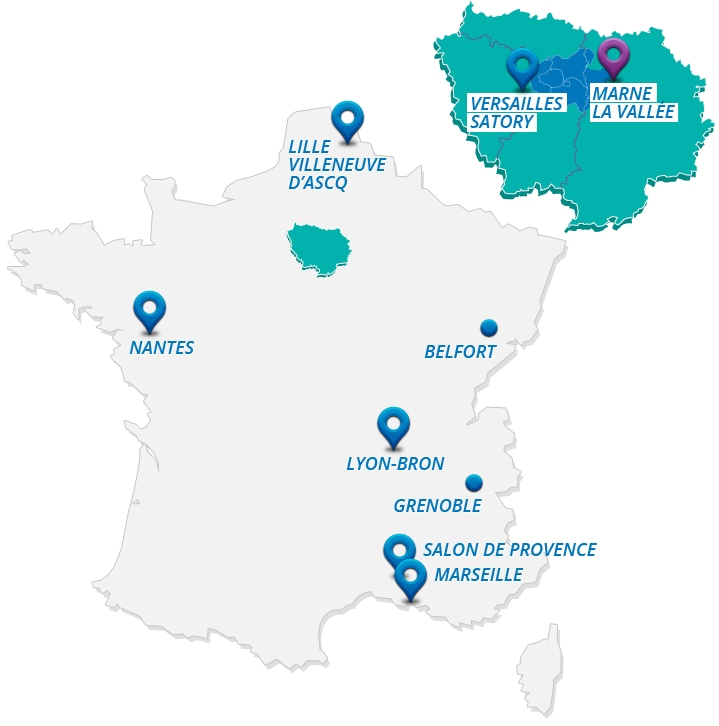
\includegraphics[height=25em]{contextualisation_du_stage/carte_sites_ifsttar}
  \caption{Répartition des différents sites de l'\ifsttar}
\end{figure}

Au total, l'\ifsttar rassemble environ un millier d'agents, dont 350 chercheurs. Il y a environ 380 doctorants accueillis dans les laboratoires de l’\ifsttar. L'\ifsttar comporte 5 départements de recherche distincts (voir annexe A). Par ailleurs, l’\ifsttar dispose d’un large patrimoine d’équipements scientifiques, qui lui permet de développer une recherche et une expertise de haut niveau. En effet, il s’agit d’équipements rares qui permettent à l’\ifsttar de conduire des travaux de recherche. Ces équipements scientifiques  sont très diversifiés : des sites et plateformes d'expérimentation, des simulateurs, des véhicules instrumentés, ou encore des recueils de données. Une importante production scientifique (thèses, publications, rapports de recherche) découle de ces équipements indispensables aux structures de recherche pour la mise en œuvre de leurs travaux.

  \subsection{Le site de Bouguenais}

\begin{figure}
  \centering
  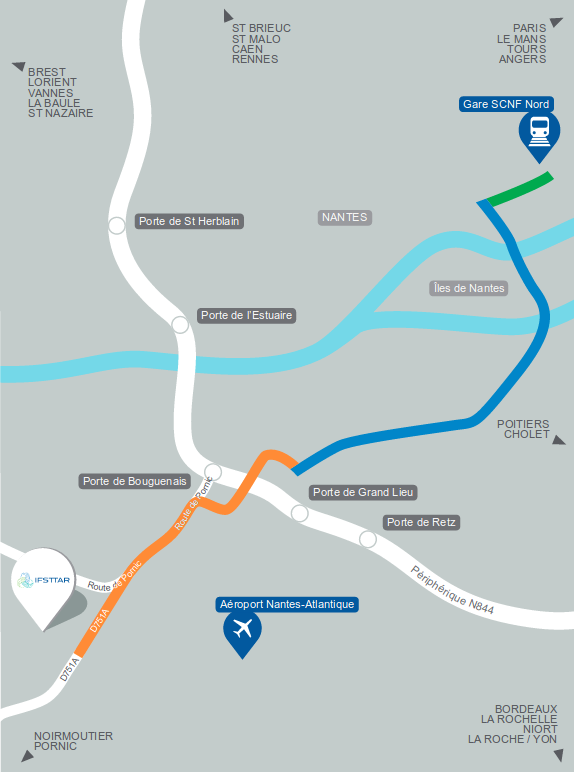
\includegraphics[height=25em]{contextualisation_du_stage/plan_acces_site_bouguenais}
  \caption{Plan d'accès du site de Bouguenais}
\end{figure}

Il y a 12 laboratoires représentant 4 départements sur le site de Bouguenais.

\begin{figure}
  \centering
  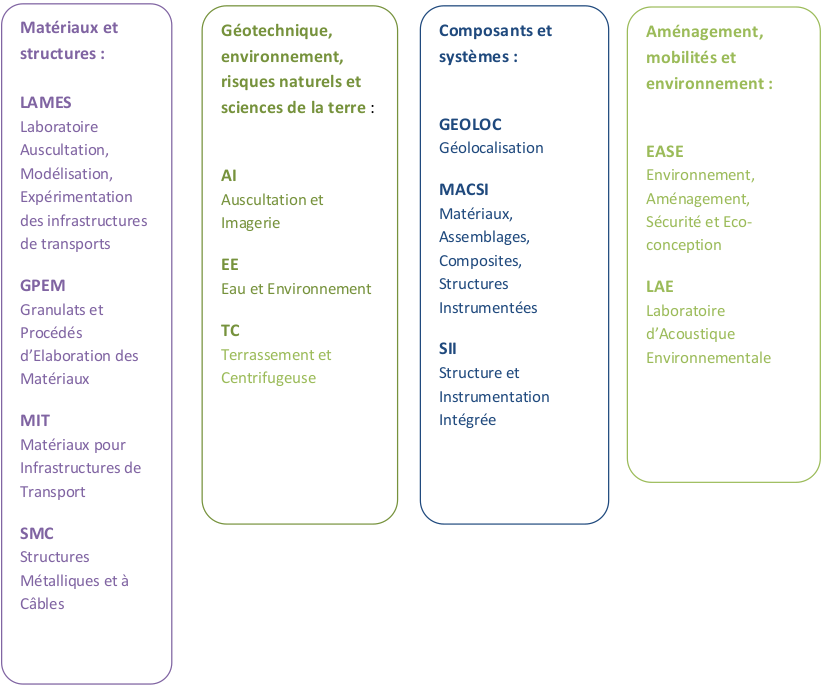
\includegraphics[height=25em]{contextualisation_du_stage/laboratoires_site_bouguenais}
  \caption{Laboratoires présents sur le site de Bouguenais}
\end{figure}


\section{Environnement et outils de travail}
  \subsection{Laboratoire d'accueil}

J'ai été accueilli au sein du laboratoire "Environnement, Aménagement, Sécurité et Eco-conception"(\bsc{EASE*}) du département "Aménagement, mobilités et environnement" (\bsc{\gls{AME}}*). Au sein du bâtiment, j'ai également été en contact avec des personnes du laboratoire (\bsc{\gls{LAMES}}*) du département "Matériaux et structures".

  \subsection{Ressources matérielles et logicielles à disposition}

J'avais bien entendu un bureau à disposition. J'avais également à disposition un tableau blanc qui m'a beaucoup servi pour les activités de conception, ainsi que pour réfléchir sur les problématiques qui ont pu se poser au long du projet.

Pour le développement, j'avais à disposition un ordinateur en dual boot, avec deux systèmes d'exploitation à ma disposition : Windows 7 et Ubuntu 16.04 \bsc{\gls{LTS}}*. Cependant je n'ai utilisé que Linux.

En ce qui concerne le déploiement de mon application, une machine nous a été rendue disponible en \gls{SSH}*. Ce serveur a notamment un disque ayant une capacité de stockage nécessaire pour traiter d'importants ensembles de données.

  \subsection{Outils utilisés}

Je me suis muni des outils avec lesquels je suis à l'aise. Ils m'ont permis de gérer et de mener à bien mon développement de manière efficace.

\begin{description}
  \item[\gls{PyCharm}*~:] \bsc{\gls{IDE}}* en version professionnelle (licence étudiante offerte par \gls{JetBrains}*)
  \item[\gls{conda}* + \gls{pip}*~:] facilitateurs de gestion des dépendances via la création d'un environnement virtuel d'exécution
  \item[\gls{git}* + \gls{GitHub}*~:] gestionnaire de version
  \item[\gls{markdown}*~:] langage à la syntaxe enfantine pour les productions rapides de petits documents
  \item[\bsc{\gls{LaTeX}}*~:] langage de présentation utilisé pour la rédaction du cahier des charges et de ce rapport
  \item[\gls{Atom}*~:] éditeur de texte, que j'ai surtout utilisé pour le markdown et le \bsc{LaTeX}
  \item[\gls{SublimeText}*~:] éditeur de texte, utilisé en complément d'Atom
\end{description}

  \subsection{Organisation et méthodologie}

L'organisation d'équipe que l'on a suivi reprend plusieurs point importants que l'on peut retrouver en méthode agile :

\begin{itemize}
  \item des évolution rapides au niveau des spécifications~;
  \item des réunions  assez courtes avec quelques questions par personne et un tableau à disposition~;
  \item une communication permanente au sein de l'équipe sur la fonctionnalité dont le développement est à prioriser~;
  \item un développement itératif~;
  \item une version fonctionnelle de l'application à tous les stades du développement~;
  \item des tests effectués sur les fonctionnalités au fur et à mesure de l'avancement.
\end{itemize}

  \subsection{Prise de notes}

Tout au long de mon stage, j'ai tenu un journal de bord qui décrit ce que j'ai réalisé au jour le jour. Par ailleurs, j'ai conservé les liens des ressources utiles que j'ai trouvées lors de mes recherches ou que l'on a pu me signaler. Je les ai accompagnés d'une description succincte indiquant la nature des informations intéressantes que l'on peut y trouver.


\chapter{Scripts shell d'installation}
  \section{Objectif}

Avant la phase de traitement des données  vient celle de la préparation de l'infrastructure. La création de la plateforme de données géographiques se traduit par l'installation d'une base de données sur un serveur distant. Dans l'optique d'automatiser ces étapes préparatoires, plusieurs scripts ont été réalisés.

Par ailleurs, si les capacités du serveur sont adaptées à exécuter l'application Python afin de rapatrier les données, il serait néanmoins possible d'exécuter le programme sur une machine client. Cela motive le choix de séparer le script de préparation de la base de données, du script de préparation de l'environnement d'exécution. Ainsi, on peut les lancer indépendamment : le premier sur le serveur de données et le second sur la machine où le code Python s'exécutera. La création de ces deux scripts répond donc à la problématique suivante. Comment effectuer facilement l'ensemble des installations nécessaires, de manière automatisée ?

Enfin, un dernier script, qui n'est pas à destination de l'utilisateur final, à été réalisé. Il permet de générer à nouveau l'environnement virtuel conda.

\section{Détail des différents scripts}

  \subsection{Installation et configuration de PostgreSQL}

Ce script, développé en bash, a pour rôle d'installer et de configurer correctement PostgreSQL. C'est le premier script à lancer lors d'une installation à partir de zéro. Il se charge notamment :

\begin{itemize}
  \item de définir les modes d'authentification~;
  \item d'autoriser les connexions à distance~;
  \item d'ajouter la journalisation des connexions et déconnexions~;
  \item d'ajouter le support de l'\bsc{\gls{UTF-8}}* par défaut~;
  \item de créer les extensions~;
  \item de créer deux rôles (lecture et écriture)~;
  \item d'assigner un mot de passe à l'utilisateur "postgres"~;
  \item de créer la base de données, vide.
\end{itemize}

En ce qui concerne les installations, ce sont de simples appels à la commande \code{apt-get}. L'ajout des rôles et du mot de passe pour l'utilisateur postgres, la création de la base et des extensions ainsi que le support de l'\bsc{UTF-8} est assez simple. Ce sont des requêtes \bsc{SQL} soumises à la base à l'aide du client \code{psql}.

En revanche, la configuration des méthodes d'authentification, l'autorisation des connexions à distance, ainsi que la configuration de la journalisation s'effectuent moins facilement. En effet, il est nécessaire de modifier deux fichiers de configuration dans le dossier \code{/etc/postgresql/9.6/main}~:

\begin{description}
  \item[\code{postgresql.conf}~:] paramètres généraux
  \item[\code{pg\_hba.conf}~:] règles d'authentification
\end{description}

Heureusement, de nombreuses commandes bash existent afin de traiter des données textuelles. Ainsi, l'utilisation de \code{sed} combinée aux expressions régulières (\code{gls{regex}}*) permet d'éditer comme souhaité ces deux fichiers de configuration.

  \subsection{Préparation de l'environnement d'exécution}

Ce script, développé en bash, a pour rôle de préparer l'environnement dans lesquels l'applicatif Python s'exécutera. C'est le second script à lancer lors d'une installation à partir de zéro. Il se charge notamment~:

\begin{itemize}
  \item de changer les permissions sur la racine de travail qui va être utilisée par le code Python~;
  \item d'installer le paquet \code{p7zip}~;
  \item d'installer miniconda~;
  \item d'importer puis d'activer l'environnement conda.
\end{itemize}

Afin d'éviter tout incident lors du lancement de l'application Python, ce script vient, en amont, effectuer les ajustements nécessaires. En effet, par défaut, le programme va travailler dans \code{/srv}, qui est un emplacement approprié pour recevoir et stocker des données vouées à être partagées. On spécifie donc des droits permissifs sur ce répertoire.

L'installation du paquet \code{p7zip} permet d'obtenir l'exécutable qui gère le format de compression \code{.7zip}. L'exécutable en question (\code{7zr}) sera appelé indirectement par le programme via la bibliothèque \code{patool}.

\code{Miniconda}, quant à lui, s'installe à partir d'un script qui est téléchargé. Il est ensuite ajouté au path, configuré, puis mis-à-jour. Tout est alors prêt pour la dernière étape, très simple, qui consiste à importer l'environnement virtuel conda. Celui-ci a été généré au préalable et est fourni dans l'arborescence du projet.

De cette manière, une fois ce script exécuté, l'ensemble des installations sont terminées.

  \subsection{Création d'un environnement virtuel conda}

Ce script est à destination des personnes souhaitant étoffer le projet à posteriori. Exécuté sur une machine ayant conda d'ores-et-déjà installé, il recrée et exporte l'environnement virtuel conda.

Voici un exemple élagué qui montre à quoi peut ressembler le fichier \bsc{\gls{YAML}}* de l'environnement conda exporté.

\begin{figure}
\centering
  \begin{lstlisting}
    name: gd
    channels: !!python/tuple
    - conda-forge
    - defaults
    dependencies:
    - conda-forge::fiona=1.7.6=np112py35_0
    - conda-forge::json-c=0.12=0
    - conda-forge::pcre=8.39=0
    - conda-forge::pip=9.0.1=py35_0
    - conda-forge::psycopg2=2.7.1=py35_0
    - conda-forge::python=3.5.3=3
    - conda-forge::readline=6.2=0
    - conda-forge::shapely=1.5.17=np112py35_2
    - conda-forge::xlrd=1.0.0=py35_1
    - util-linux=2.21=0
    - pip:
      - patool==1.12
    prefix: /home/taunay/miniconda/envs/gd
  \end{lstlisting}
\caption{Environnement virtuel conda exporté (simplifié)}
\end{figure}

Cela permet de faciliter l'ajout ultérieur d'une bibliothèque. En effet, il suffit d'ajouter le paquet nécessaire au sein du script et de le lancer. De cette manière, l'environnement virtuel conda nouvellement généré comportera la ou les bibliothèques ajoutées.


\chapter{Interactions utilisateur : fichiers de configuration}
  \section{Rôle des fichiers de configuration}

Les fichiers de configuration sont au cœur du fonctionnement du logiciel. Renseignés par l'utilisateur, ils formalisent le traitement souhaité sur les données ainsi que leur conditions d'import. On peut donc énoncer les points nécessaires que doivent respecter les fichiers de configuration. Ainsi, l'utilisateur doit être en mesure, à travers ces fichiers :

\begin{itemize}
  \item d'exprimer simplement les pré-traitements et les conditions d'import;
  \item de spécifier le tout de manière assez formalisée afin que le fichier, ensuite lu par le programme, ne soit pas ambigü;
  \item d'omettre des informations lorsque c'est possible, ce qui correspond à une délégation implicite au programme de certaines tâches.
\end{itemize}

\section{Profil utilisateur}

L'utilisateur final doit répondre à certains critères. Ces prérequis permettent de vérifier que l'utilisateur sera en mesure d'utiliser correctement le programme en suivant simplement le manuel utilisateur.

Ainsi l'utilisateur doit être capable, au minimum, d'utiliser basiquement la ligne de commande. C'est souhaitable afin de pouvoir lancer les scripts. Il doit également, si possible, être apte à naviguer dans l'arborescence voire effectuer des manipulations courantes sur les fichiers (déplacement, édition).

De cette manière, le logiciel peut tout-à-fait être utilisé par une personne qui ne développe pas.

\section{Fichier général de configuration}

Ce fichier, séparé des paramètres d'import spécifiques à chaque donnée, contient les paramètres communs à toutes les données. Ils sont d'une importance très variables : caractère visuel de séparation utilisé par les logs et \bsc{\gls{IP}}* de la base de données, par exemple.

Dans un logiciel graphique, on peut se représenter ce fichier de configuration comme étant la version \bsc{JSON} de l'onglet "préférences" ou "options".

\section{Fichier JSON de configuration des imports}
    \subsection{Définition d'un import}

  Ce fichier a pour vocation de permettre à l'utilisateur de définir les données à importer et les traitements souhaités sur celles-ci. Face au grand nombre de sources de données qui peuvent être précisées par l'utilisateur, le défi ici consiste à construire une configuration assez souple. En effet, seule le strict nécessaire doit être précisé par l'utilisateur. En procédant de cette manière et à force de faire évoluer ce fichier de configuration, nous avons aboutit à un fichier semblable à l'exemple présenté ci-contre.

  \begin{figure}
    \centering
    \begin{lstlisting}
      "res": {
        "import_mode": "controlee_nouvelle_table",
        "params": {
          "shortname": "epci_lamb93_2013",
          "data_name": "epci-20131220-5m",
          "uri": "https://osm13.openstreetmap.fr/.../epci-20131220-5m-shp.zip",
          "schema": "geofla",
          "table": "epci_lamb93",
          "year": 2013,
          "version": "epci_osm_2013",
          "srid_source": 4326,
          "srid_destination": 2154,
          "bindings": [
            {"from": "nom_epci", "type": "str:64", "to": "libelle_epci"},
            {"from": "ptot_epci", "type": "", "to": ""}
          ],
          "mode":"modified"
        }
      }
    \end{lstlisting}
    \caption{Exemple de fichier de configuration des imports}
  \end{figure}

Sur cet l'exemple ci-contre, un champs de la donnée d'entrée est renommé, un est supprimé, et les autres sont conservés en l'état. En effet, un \code{"to"} vide est synonyme de suppression. Le mode \code{"modified"} précise que les autres attributs seront conservés. Il s'oppose au mode \code{"keep\_only"} qui lui ne conservera que les champs \code{"from"} précisés dans la node \code{"bindings"}.

Ce type de souplesse permet de limiter le nombre de champs à renseigner. En effet, il serait extrêmement contraignant pour l'utilisateur d'avoir à préciser l'ensemble des attributs alors que seul quelques champs seront renommés ou laissés de côté. Dans le cas des données que l'on traite ici, l'intérêt est de taille car certaines données ont un nombre assez important d'attributs.

    \subsection{Problème soulevé}

Le fichier \bsc{JSON} de configuration des imports permet de renseigner les imports à effectuer. Cependant, même muni d'un éditeur de texte approprié, éditer un fichier \bsc{JSON} pour y ajouter de nombreux imports présente un certain nombre d'inconvénients non négligeables.

\begin{itemize}
  \item Les sources d'erreurs au niveau du formatage dûes aux copier-coller sont nombreuses : il est facile d'oublier une virgule ou une accolade fermante.
  \item Le format \bsc{JSON}, bien que décemment espacé et indenté, ne permet pas une vue d'ensemble satisfaisante : il est difficile pour l'utilisateur de se repérer au sein du fichier.
\end{itemize}

C'est pourquoi il a fallu trouver une réponse à ces problématiques, c'est-à-dire un autre moyen de saisie de l'entrée utilisateur.

    \subsection{Solution : fichier tableur et script de conversion}

Le choix de ce moyen de saisie s'est porté sur une feuille de tableur, par souci de simplicité et de commodité. Une fois sa syntaxe fixée après une phase de concertation, il fallait pouvoir obtenir un fichier de configuration \bsc{JSON} à partir de ce fichier.

Le script \code{excel2conf.py} vient remplir ce rôle. Il prend en entrée un ensemble de chemins absolus pointant vers des fichiers excel contenant les informations sur les imports à effectuer. Ce script va produire, pour chacun de ces fichiers tableur un équivalent \bsc{JSON}. Les fichiers \bsc{JSON} alors produits pourront ensuite être fournis au système de la même manière qu'un fichier d'import réalisé manuellement.

Afin de mener à bien cette tâche, le script se repose sur la bibliothèque \code{xlrd}, qui lui permet de parcourir le fichier tableur. De cette manière, chaque feuille correspondant à un mode d'import valide (nouvelle table ou table existante) est parcourue. Au sein de ces feuilles, chaque ligne correspond à un import. Il devient alors très visuel et facile de remplir les imports souhaités. Cette solution se révèle d'autant plus satisfaisante lorsque le nombre de données à importer augmente.

Enfin, il est possible, et judicieux, de vérifier les fichiers \bsc{JSON} produits par le script avant de les fournir au programme. En effet, il arrive que certaines erreurs, difficilement remarquables au sein du tableur, apparaissent de façon beaucoup plus flagrante en \bsc{JSON}. On peut par exemple pointer du doigt les sauts de ligne issus de copier-coller, bien visibles en tant qu'\code{\textbackslash n} dans le fichier de configuration \bsc{JSON} produit.

\section{Fichier répertoriant les imports effectués}

Une fois un fichier de configuration des imports obtenu et le programme principal lancé, toutes les données correspondant aux entrées du fichier de configuration des imports n'ont pas toutes subi le même traitement. Par exemple, l'\gls{URI}* fournie par l'utilisateur peut tout à fait être momentanément inaccessible ou erronée. De ce fait, chaque ressource aboutit à un stade final qui lui est propre :

\begin{itemize}
  \item non récupérée, ressource inaccessible via l'URI renseignée~;
  \item récupérée avec succès, mais format de compression non géré par un exécutable, disponible sur le système, auxquel la bibliothèque \code{patool} puisse faire appel~;
  \item récupérée et extraite, mais donnée souhaitée introuvable au sein de l'arborescence~;
  \item succès du parsage, des modifications structurelles et de la construction des requêtes mais échec au niveau de l'import en base de données~;
  \item chaîne complète de succès aboutissant à un import effectif en base de données.
\end{itemize}

La cause d'un échec fait l'objet de détails dans les logs, ce qui permet de la corriger avant le lancement suivant. Dès lors, la reprise s'effectuera à partir de la dernière étape réussie. C'est très facile de connaître le statut en se basant sur le système de fichiers pour les étapes de téléchargement de de décompression.

Cependant ce n'est pas le cas pour l'étape d'import en base. Afin de palier à ce problème, un fichier, accessible à l'utilisateur est placé dans le même répertoire que le fichier de configuration des imports. Il retient chaque donnée importée, ce qui permettra à l'utilisateur de connaître facilement les imports finalement effectués. De même, s'il a besoin d'importer à nouveau une donnée il lui suffit de supprimer la ligne correspondant à cette donnée au sein de ce fichier.


\chapter{Applicatif Python}
  \section{Présentation générale du problème}

Les scripts d'installation ont répondu, en partie, à la problématique générale posée initialement : construire, à partir de zéro, une base de données géoréférencées. En effet, ce sont les installations automatisées qui vont permettre de "partir de zéro". Vient dorénavant la question de  l'import des données qui vont venir alimenter cette base de données géoréférencées.

Les données géoréférencées qui nous intéressent ici sont hétérogènes et de qualité variables. En effet les données à disposition sont mises en ligne par différents organismes. On peut citer par exemple l'\bsc{\gls{INSEE}}*, l'\bsc{\gls{IGN}}*, OpenStreetMap ou encore la \bsc{\gls{CAF}}*. Cela induit le fait que les données peuvent être contenues dans des fichiers de formats variables comme le format \code{.shp}, le plus répandu, ou encore les formats \code{.mif/.mid} et \code{.geojson}. On trouve même des données, moins sujettes à du traitement automatique, par exemple des feuilles excel \code{.xls}. La variété des formalismes de chaque organisme rend difficile ces données à traiter, d'où l'intérêt de la création d'une base de données géoréférencées.

Vient ensuite l'aspect géoréférencé des données : ils donnent lieu à des traitements spécifiques. En effet, il peut être nécessaire de reprojeter des données afin que les données soient homogènes au sein d'une même table en base. L'extension PostGIS, dans sa table \code{spatial\_ref\_sys}, répertorie plus de 5000 projections différentes. Enfin, la colonne \code{geometry} gérant l'aspect géoréférencé des données d'entrée n'est pas à même d'être importée en base en l'état : la représentation attendue par PostGIS diffère.

\section{Finalité du projet}

L'applicatif Python constitue l'outil principal, il est au cœur du projet. L'application à concevoir et développer devra permettre de répondre au problème posé, c'est-à-dire de remplir une base de données géoréférencées. Les imports en base doivent pouvoir être effectués de manière souple, mais contrôlée.

De plus, les imports devront pouvoir s'effectuer de manière assistée, où les différentes actions effectuées ainsi que les problèmes rencontrés devront être indiqués.

Enfin, la mise en œuvre de l'application permet d'omettre certains paramètres dans les fichiers de configuration d'import. En cela, le programme est automatisé. Néanmoins, il reste soumis à la demande de l'utilisateur : le script n'est pas voué à se lancer tout seul à intervalles régulièrs, à l'aide de \code{cron} par exemple. Les tâches de vérification de nouvelles parutions de données restent manuelles. Ainsi les données stockées au sein de la base peuvent être mises-à-jour ou non au bon vouloir de l'utilisateur. C'est seulement alors qu'interviendra l'utilisateur afin de préciser les imports qu'il souhaite effectuer.

\section{Fonctionnalités attendues}
  \subsection{Paramétrabilité et facilité d'utilisation}

L'utilisateur ne fait que déléguer à l'application les traitements à effectuer, ce qui ne le dispense pas de renseigner des paramètres afin de guider le programme. Les fichiers de configuration viennent répondre à ce besoin.

La principale contrainte pour ceux-ci est qu'ils doivent être à la fois concis, c'est-à-dire qu'il y ait le moins d'informations possible à renseigner par l'utilisateur~; mais aussi complets, c'est-à-dire que l'utilisateur puisse donner exactement ce qu'il souhaite.

Enfin, afin de faciliter l'utilisation du programme, un manuel utilisateur a été rédigé (voir annexe B). Il guide l'utilisateur et lui permet de s'orienter au sein du projet.

  \subsection{Journalisation des actions effectuées}

La clarté d'exécution est un critère particulièrement important et attendu. De ce fait, une attention toute particulière à été portée sur ce point. C'est pourquoi les logs de l'application se veulent les plus clairs possibles. Le défi ici est d'être assez précis et concis, tout en restant assez général afin que l'utilisateur final ne se perde pas dans les détails pour autant.

Au sein du code source, cela se traduit par une vérification constante assez fine quant aux retours des fonctions clés de traitement. Ainsi, ces fonctions retournent un paramètre supplémentaire, indiquant à leur fonction appelante la réussite ou l'échec du traitement demandé, le cas échéant. La fonction appelée se sera alors chargée, si nécessaire, de produire une ligne de journalisation détaillant le problème rencontré pour cet appel.

\begin{Code}
  def log(msg, lvl='info'):
      """
      Journalise les evenements de maniere formatee.

      Les messages seront prefixes du niveau de severite.
      Le LOG_LEVEL precise l'importance moindre a partir de laquelle afficher le message.
      :param msg: string le message
      :param lvl: string le niveau
      """

      def print_it():
          printerr('[{}] {}'.format(lvl.upper(), msg))

      levels_to_print = SEVERITY_LEVELS[:SEVERITY_LEVELS.index(LOG_LEVEL)+1]

      if lvl in levels_to_print:
          print_it()

      # niveau special non defini par defaut
      # on affiche donc le message independemment du LOG_LEVEL
      if lvl not in SEVERITY_LEVELS:
          print_it()
\end{Code}

La principale fonction de journalisation, appelée à de nombreuses reprises au sein de l'exécution est détaillée ci-contre. On peut notamment remarquer la présence d'une configuration du niveau de gravité minimum à partir duquel afficher un log. Cela permet, par exemple, si l'utilisateur effectue un grand nombre d'imports simultanément, d'être en mesure de ne visualiser que les entrées de journalisation d'erreur et de mise en garde, s'il le souhaite.

  \subsection{Récupération des données}

Le récupération des données s'effectue différemment en fonction des \bsc{URI}. En effet, le traitement se distingue entre les ressources locales (\bsc{URI} en \code{file:///}) et les ressources web distantes (\bsc{URI} en \code{http}). Pour les données accessibles en local, elles sont simplement copiées dans l'arborescence de travail du programme. Les ressources distantes sont téléchargées via des appels aux fonctions d'\code{urllib}.

\begin{Code}
  with open(save_as, 'wb') as output_file:
      response = get(uri, verify=False)
      output_file.write(response.content)
\end{Code}

Afin de pouvoir se déplacer manuellement dans les données téléchargées à des fins de consultation, copie ou partage, il est nécessaire que ces données soient correctement agencées. L'arborescence est tout d'abord découpée selon chaque site de téléchargement. Les données copiées sont dans un dossier "\code{copied}" dans ce même répertoire. Puis, chaque dossier de site se découpe en nom de données téléchargées. Il y en a un par archive distincte.

En procédant de la sorte, il est facilement possible de savoir si une donnée a d'ores-et-déjà été téléchargée. En effet, le chemin vers l'emplacement attribué à cette donnée fait office de clé. Il suffit alors de constater la présence ou l'absence de l'archive en question.

  \subsection{Décompression des archives}

Les données mises à disposition par les différentes institutions sont fournies comme archives. On trouve surtout des \code{.zip} et \code{.7z}. La bibliothèque \code{patool} permet conserver un traitement standard pour tous les formats au niveau du code source de l'application. Cette bibliothèque se charge en réalité d'appeler l'exécutable sur le système approprié pour décompresser l'archive, après détection du type \bsc{\gls{MIME}}* de celle-ci.

En se basant sur \code{patool}, j'ai donc défini une fonction de test pour déterminer si un fichier est constitutif ou non d'une archive.

\begin{Code}
  def is_archive(params):
      """
      Determine si le fichier passe en parametre est une archive.

      :param params: les parametres
      :return: True si c'est une archive, False sinon
      """
      try:
          test_archive(params['path'], verbosity=-1, interactive=False)
      except Exception:
          return False
      return True
\end{Code}

Cette fonction sert à sélectionner les archives lors de la recherche des archives à décompresser~:

\begin{Code}
    archives_to_extract = search_with_criteria(DOWNLOAD_ROOT, is_archive, search_depth=2)
\end{Code}

La bibliothèque \code{patool} permet ensuite d'extraire chaque archive en fournissant uniquement son chemin, comme suit.

\begin{Code}
  extract_archive(archive_path, verbosity=-1, outdir=archive_dir, interactive=False)
\end{Code}

  \subsection{Recherche d'une donnée}

Une problématique s'est posée lors de la recherche des données au sein des archives décompressées ayant été téléchargées. En effet, il s'est avéré que certains organismes regroupent plusieurs données au sein d'une même archive ressource. Il est donc fréquent d'observer plusieurs données au sein d'une même archive. Ces données peuvent être un fichier unique ou un ensemble de fichiers.

Deux cas de figures se présentent~:
\begin{itemize}
  \item L'utilisateur a renseigné le nom de la donnée de manière précise, c'est-à-dire le nom du ou des fichier(s).
  \item L'utilisateur a omis le nom de la donnée.
\end{itemize}

Dans le premier cas, il suffit d'utiliser ce nom au sein de la recherche. Ci-contre le code source de la fonction utilitaire de recherche récursive avec critère. Le \code{validator} qui sera passé ici est une fonction renvoyant un booléen. Ce booléen vaut \code{True} si le fichier correspondant au chemin absolu passé en paramètre correspond à un fichier qui nous intéresse, \code{False}.

\begin{Code}
  # Prototype de la fonction de recherche recursive avec criteres.
  def search_with_criteria(path_to_search_in, validator, validator_params=None, search_depth=0):
  """Recherche les fichiers satisfaisant un ensemble de critères au sein du dossier specifie."""
\end{Code}

La distinction avec le second cas s'exprime donc au niveau de la fonction de validation passée en paramètre. Si le nom précis de la donnée n'est pas renseigné, l'algorithme de recherche ne se basera que sur les extensions de fichiers afin de trouver des groupes intéressants de fichiers. Si plusieurs groupes sont trouvés, alors le traitement pour cette donnée s'arrête là. En effet, le programme avertit l'utilisateur que le nom de la donnée doit impérativement être renseigné pour cet import. Néanmoins, il n'y aura souvent qu'une seule et unique donnée potentielle au sein d'une archive. C'est pourquoi cette souplesse qui permet de ne pas renseigner le nom de la donnée est essentielle puisqu'elle épargne à l'utilisateur cette action.

  \subsection{Modification de leur structure}

Les fichiers sont ouverts à l'aide de la bibliothèque \code{fiona}. Cette bibliothèque se concentre sur la lecture et l'écriture de donnée. Ce n'est pas elle qui est à même de gérer des transformations géographiques, par exemple. Cette bibliothèque permet notamment de lire un bon nombre de fichiers qui contiennent des données géoréférencées et de construire une structure python, en l'occurrence un dictionnaire, qui les représente en mémoire.

De plus, \code{fiona} permet de travailler avec les données en flux, ce qui est essentiel au vu de l'importante volumétrie des données que l'on traite ici. En effet, il est possible, en fonction du système sur lequel sera lancé l'application, que certains fichiers de données à importer soient trop conséquent pour être chargé en mémoire vive (\bsc{\gls{RAM}}*). De ce fait, le traitement en flux revête toute son importance.

L'utilisateur peut préciser, au sein du fichier de configuration des imports, un certain nombre de modifications structurelles. Il peut aisément spécifier les actions suivantes~:

\begin{description}
  \item[renommage~:] modifier le nom d'un attribut~;
  \item[filtrage~:] ne conserver que les attributs qu'il spécifie~;
  \item[suppression~:] supprimer des attributs qu'il spécifie~;
  \item[choix] déterminer le comportement du logiciel pour cette donnée, le "mode".
\end{description}

Le mode aura pour valeur \code{"modified"} ou \code{"keep\_only"}. Dans le premier cas, les attributs non spécifiés par l'utilisateur seront conservés en l'état, sans aucune action de la part du logiciel. Dans le second cas, les attributs non spécifiés seront jetés.

  \subsection{Reprojection de jeux de données}

Il arrive que des données que l'on souhaite ajouter à une table existante en base soient projetées dans un système de référence spatiale différent. Chacun de ces systèmes est associé a un identifiant unique, son \bsc{\gls{SRID}}*. Le \bsc{SRID} source ainsi que le \bsc{SRID} de destination de la table doivent tous les deux à renseigner dans le fichier de configuration des imports.

Néanmoins, si les données le permettent (présence d'un fichier \code{.prj}), le logiciel doit pouvoir détecter la projection source. De même, il doit détecter le \bsc{SRID} de destination via une introspection de la table désirée pour l'import.

Une fois les \bsc{SRID} source et destination connus, la bibliothèque \code{pyproj} pourra par exemple être utilisée.

  \subsection{Importation en base}

À l'aide la bibliothèque \code{psycopg}, il est très simple de se connecter au \bsc{SGBD} PostgreSQL~:

\begin{Code}
  connect(host=DB_HOST, port=DB_PORT, dbname=DB_NAME, user=DB_USER_NAME, password=DB_USER_PASSWORD)
\end{Code}

La fonction \code{connect()} renvoie une connexion vers la base de données. Pour effectuer une requête, on peut procéder comme suit~:

\begin{Code}
  cur = conn.cursor()
  cur.execute(query)
  conn.commit()
\end{Code}

Par ailleurs, les données sont traitées en flux. À partir de chaque entrée d'un fichier d'entrée, c'est-à-dire pour chaque futur tuple en base de données, le logiciel construit dynamiquement une requête d'insertion à envoyer en base de données, puis l'envoie.

\begin{Code}
  def build_insert_query(properties, params):
      """Construit une requete d'insertion dans une table a partir d'une feature donnee."""

      # valeurs intermediaires
      columns = list(properties.keys())
      wkt = shape(properties['geometry'])
      srid = params['srid_source']
      geometry_field = "ST_GeomFromText('{}', {})".format(wkt, srid)

      # champs pour requetes
      table_name = '"{}"."{}"'.format(params['schema'], params['table'])
      fields_list = '({})'.format(', '.join(columns))
      values = '({})'.format(', '.join([geometry_field if attr == GEOMETRY_NAME else "'{}'".format(p.replace("'", "''")) if isinstance(p, str) else str(p) for attr, p in properties.items()]))

      query = 'INSERT INTO {} {} VALUES {};'.format(table_name, fields_list, values)

      return query
\end{Code}

Cette construction des requêtes d'insertion, dont la fonction est détaillée ci-contre, permet de mettre en évidence le traitement spécifique réalisé pour l'aspect géoréférencé des données. En effet, la colonne nommée \code{geometry} des données d'entrées --- ici, une clé au sein du dictionnaire délivré par \code{fiona} --- n'est pas de la forme attendue par l'extension PostGIS, côté base de données. En effet, la représentation de l'attribut \code{geometry} dans PostGIS diffère de celle qui est attendue. Cependant, on ne peut l'obtenir directement.

Le Well-Known Text (\bsc{\gls{WKT}}*) est un format standard qui sert d'intermédiaire. En effet, du côté base de données, l'appel à \code{ST\_GeomFromText} permet de transformer les données afin de pouvoir les stocker dans la colonne \code{geometry}, à partir du well know text. Ainsi, côté Python, il faut obtenir le \bsc{WKT}. Comme on peut le voir ici, c'est à l'aide de la fonction \bsc{shape()} de la bibliothèque \bsc{shapely} que le logiciel obtient le \bsc{WKT} à partir des données d'entrée.

  \subsection{Comportement intelligent}

Un comportement dit "intelligent" est attendu. Lors de la recherche d'une donnée, le nom du fichier souhaité pouvait être omis par l'utilisateur afin que le programme le détecte de lui-même. C'est un exemple de comportement "intelligent".

De même, le logiciel produit des avertissements. Ceux-ci n'interrompent pas le traitement, mais font état d'un petit problème qui a été rencontré. En effet, il avertit l'utilisateur lorsque les fichiers de configuration comportent des fautes mineures de formatage ou de logique au sein du fichier de configuration des imports~:

\begin{itemize}
  \item l'utilisateur a renseigné une clause "drop" alors que le mode est "keep\_only", c'est un non-sens qui est signalé car il est inutile de renseigner un attribut à retirer qui sera de toute manière laissé de côté~;
  \item l'utilisateur a renseigné un nom peu approprié pour un dossier de stockage d'une donnée à récupérer~; un nom corrigé est alors suggéré.
\end{itemize}

Enfin, il est inconfortable de retirer du fichier de configuration les données ayant d'ores-et-déjà été traitées. De ce fait, le programme ne téléchargera pas à nouveau une donnée ayant déjà été téléchargée. Il en va de même au sujet des imports en base de données.


\chapter*{Conclusion}
  \addcontentsline{toc}{chapter}{Conclusion}

\section*{État de l'avancement du projet}
  \addcontentsline{toc}{section}{État de l'avancement du projet}

Le logiciel réalisé permet de répondre au besoin général initialement énoncé, à savoir créer, facilement et à partir de zéro, une base de données géographiques. Des scripts permettent d'effectuer automatiquement les installations et configurations adéquates. Finalement, le programme principal permet de :

\begin{itemize}
  \item récupérer les données à traiter (téléchargement)~;
  \item décompresser les archives récupérées~;
  \item explorer ces données afin d'en trouver la donnée intéressante~;
  \item parser ces données (supporté pour un nombre limité de formats)~;
  \item y appliquer les pré-traitements nécessaires~;
  \item les importer en base.
\end{itemize}

L'ensemble des fonctionnalités implémentées ont été testées manuellement. J'ai cherché à éprouver les cas spécifiques. Ainsi j'ai notamment vérifié le comportement de l'application pour différentes configuration d'import.

\section*{Limites de l'outil principal développé}
  \addcontentsline{toc}{section}{Limites de l'outil principal développé}

Il est important de mettre en avant que l'application en elle-même n'est pas limitée par la taille des données. En effet, l'ensemble des traitements s'effectuant en flux, la capacité du système en mémoire vive ne pose pas de problème.

Seule la capacité de stockage en mémoire morte des données d'entrée peut constituer un facteur limitant. par ailleurs la qualité de la connexion internet influe beaucoup sur la durée de rapatriement des données, puisque la majorité des ressources sont des ressources distantes. Ainsi la vitesse de traitement est environ linéaire par rapport au volume des données d'entrée.

En ce qui concerne la structure générale du projet, le choix d'avoir développé les différents modules en les rendant indépendants les uns des autres peut être critiqué sur le long terme. Certes, chacun constitue une brique réutilisable à part. Cependant, cette conception trouve ses limites car chaque module doit aller retrouver et parser les fichiers de configuration, tour à tour. Un changement de structure au niveau de ces configuration serait difficile à opérer. Cela explique le fait d'avoir fixé au plus tôt la structure de ces fichiers.

Ainsi, il aurait été possible de s'appuyer sur le paradigme de la programmation orientée objet afin de créer une classe représentant une donnée à importer. Cette dernière aurait par exemple un attribut représentant son stade actuel ; c'est-à-dire récupérée, extraite ou importée. En procédant de la sorte, un gain de modularité supplémentaire serait obtenu.

\section*{Perspectives d'amélioration}
  \addcontentsline{toc}{section}{Perspectives d'amélioration}

Les scripts shell développés respectent les bonnes pratiques de développement, mais ne se plient pas pour autant aux normes \bsc{\gls{POSIX}}*. Respecter ces contraintes au sein de ces scripts augmenterait leur portabilité.

Le développement d'une interface graphique pourrait être réalisé. Celle-ci permettrait par exemple de créer plus simplement les fichiers de configuration, de façon totalement transparente à l'utilisateur. Ainsi, le programme gagnerait énormément en interactivité et en sûreté. En effet le fichier de configuration généré serait ainsi systématiquement correct sur la question du formatage. De même, l'utilisateur pourrait avoir la possibilité d'importer en filtrant via des critères, ou de n'effectuer que l'étape de téléchargement pour une donnée par exemple. Une telle surcouche demanderait un développement assez conséquent car on peut alors imaginer beaucoup de nouvelles fonctionnalités comme ces quelques exemples.

Pour ce qui est de l'outil principal, la gestion d'un plus grand nombre de formats est un point à travailler. En effet, la diversité des sources de données, et, de façon analogique, des données qu'elles mettent à disposition est assez importante. Néanmoins il faut garder à l'esprit que la souplesse de l'application développée permet de distinguer aisément les traitement associés aux différents cas.

 \section*{Expérience acquise}
   \addcontentsline{toc}{section}{Expérience acquise}

Premièrement, j'ai constaté l'importance d'accorder une attention toute particulière aux étapes en amont de l'implémentation. Ainsi, j'ai progressé au niveau du recueil du besoin et de sa définition, mais également sur les activités de conception. En effet, au cours de l'élaboration de la solution, la majorité des problèmes potentiels ont été soulevés tôt. Cela a permis d'orienter la conception de l'application, notamment au niveau de son découpage. De cette manière, l'application est suffisamment modularisée pour gérer tous les cas : l'ensemble des traitements communs à plusieurs scénarios d'exécution sont factorisés.

De plus, ce stage a été l'occasion d'utiliser mes compétences de scripting shell en bash lors de la réalisation des scripts d'installation et de configuration.

Par ailleurs, je suis monté en compétence sur le langage Python. En particulier, j'ai été amené à manipuler plusieurs bibliothèques, énoncées ci-après. Chacune est accompagnée d'un bref descriptif de l'utilisation qui en est faite au sein du projet.

\begin{description}
  \item[patool~:] décompression en fonction du type \bsc{MIME}~;
  \item[xlrd~:] parsage du fichier excel précisant les imports~;
  \item[fiona~:] parsage des données à traiter~;
  \item[shapely~:] modifications sur la colonne geometry~;
  \item[psycopg2~:] connexion à la base de données.
\end{description}

En ce qui concerne les outils, j'ai appris à utiliser conda afin de gérer efficacement des environnements virtuels. J'ai aussi progressé sur le langage de présentation LaTeX lors de la rédaction du cahier des charges et de ce rapport.

\clearpage
\pagenumbering{gobble}


\pagenumbering{gobble}\printglossaries\clearpage
  \addcontentsline{toc}{chapter}{Glossaire}

\chapter*{Sources}
  \addcontentsline{toc}{chapter}{Sources}

{

\small

\paragraph{PostgreSQL/PostGis}
\begin{description}

  \item Comparatif MySQL et PostgreSQL \\
  \url{https://openclassrooms.com/courses/mysql-et-postgresql-lequel-choisir}

  \item Tutoriel sur les rôles et permissions \\
  \url{https://www.digitalocean.com/community/tutorials/how-to-use-roles-and-manage-grant-permissions-in-postgresql-on-a-vps--2}

  \item Gestion des droits \\
  \url{https://wiki.postgresql.org/images/d/d1/Managing_rights_in_postgresql.pdf}

  \item Introduction à PostGIS \\
  \url{http://suite.opengeo.org/docs/latest/dataadmin/pgGettingStarted/firstconnect.html}

  \item Les schémas \\
  \url{https://www.postgresql.org/docs/current/static/ddl-schemas.html}

\end{description}





\paragraph{Scripting shell}
\begin{description}

  \item Génération d'un mot de passe aléatoire \\
  \url{https://www.howtogeek.com/howto/30184/10-ways-to-generate-a-random-password-from-the-command-line/}

  \item Documentation conda \\
  \url{https://conda.io/docs/using/envs.html}

\end{description}





\paragraph{Python}
\begin{description}

  \item Tutoriel SDZ/OC \\
  \url{https://openclassrooms.com/courses/apprenez-a-programmer-en-python}

  \item Erreurs courantes au sujet des imports \\
  \url{http://python-notes.curiousefficiency.org/en/latest/python_concepts/import_traps.html}

  \item Notions basiques de manipulation de dossiers \\
  \url{http://www.diveintopython.net/file_handling/os_module.html}

  \item PEP 257 sur les docstrings \\
  \url{https://www.python.org/dev/peps/pep-0257/}

  \item PEP 343 sur le mot-clé "with" \\
  \url{https://www.python.org/dev/peps/pep-0343/}

\end{description}





\paragraph{Bibliothèques et aspect géo-référencé des données}
\begin{description}

    \item Librairie GDAL (Geospatial Data Abstraction Library) \\
    \url{http://www.gdal.org/}

    \item Spécifications GeoJSON \\
    \url{https://tools.ietf.org/html/rfc7946}

    \item Modules python à finalités géospatiales : index à tutos, récapitulatif / descriptifs \\
    \url{http://www.portailsig.org/content/les-modules-python-finalites-geospatiales-quid-quando-ubi}

    \item Coment combiner l'utilisation des bibliothèques shapely et fiona \\
    \url{https://macwright.org/2012/10/31/gis-with-python-shapely-fiona.html}

    \item Fiona, geojson, et attributs \\
    \url{https://gis.stackexchange.com/questions/41465/generating-geojson-with-python}

    \item Fiona : ajout de propriétés \\
    \url{https://gis.stackexchange.com/questions/191900/fiona-error-adding-property-to-shapefile/191953}

    \item Fiona, geojson, et projection \\
    \url{https://gis.stackexchange.com/questions/192830/fiona-does-not-specify-crs#192873}

    \item Documentation sur l'utilisation d'osgeo \\
    \url{https://pcjericks.github.io/py-gdalogr-cookbook/vector_layers.html}

    \item Documentation pyproj \\
    \url{https://jswhit.github.io/pyproj/}

\end{description}





\paragraph{Rédaction du rapport}
\begin{description}

  \item Tutoriel SDZ/OC \\
  \url{https://openclassrooms.com/courses/redigez-des-documents-de-qualite-avec-latex}

  \item Compilation de conseils \\
  \url{http://enicolashernandez.blogspot.fr/2011/03/redaction-dun-rapport-de-stage.html}

  \item Données chiffrées et ressources visuelles \\
  \url{http://www.ifsttar.fr/accueil/}

\end{description}

}

\clearpage


\chapter*{Annexes}
  \addcontentsline{toc}{chapter}{Annexes}

\section*{A. Organigramme des départements de l'\ifsttar}
  \addcontentsline{toc}{section}{A. Organigramme des départements de l'\ifsttar}
  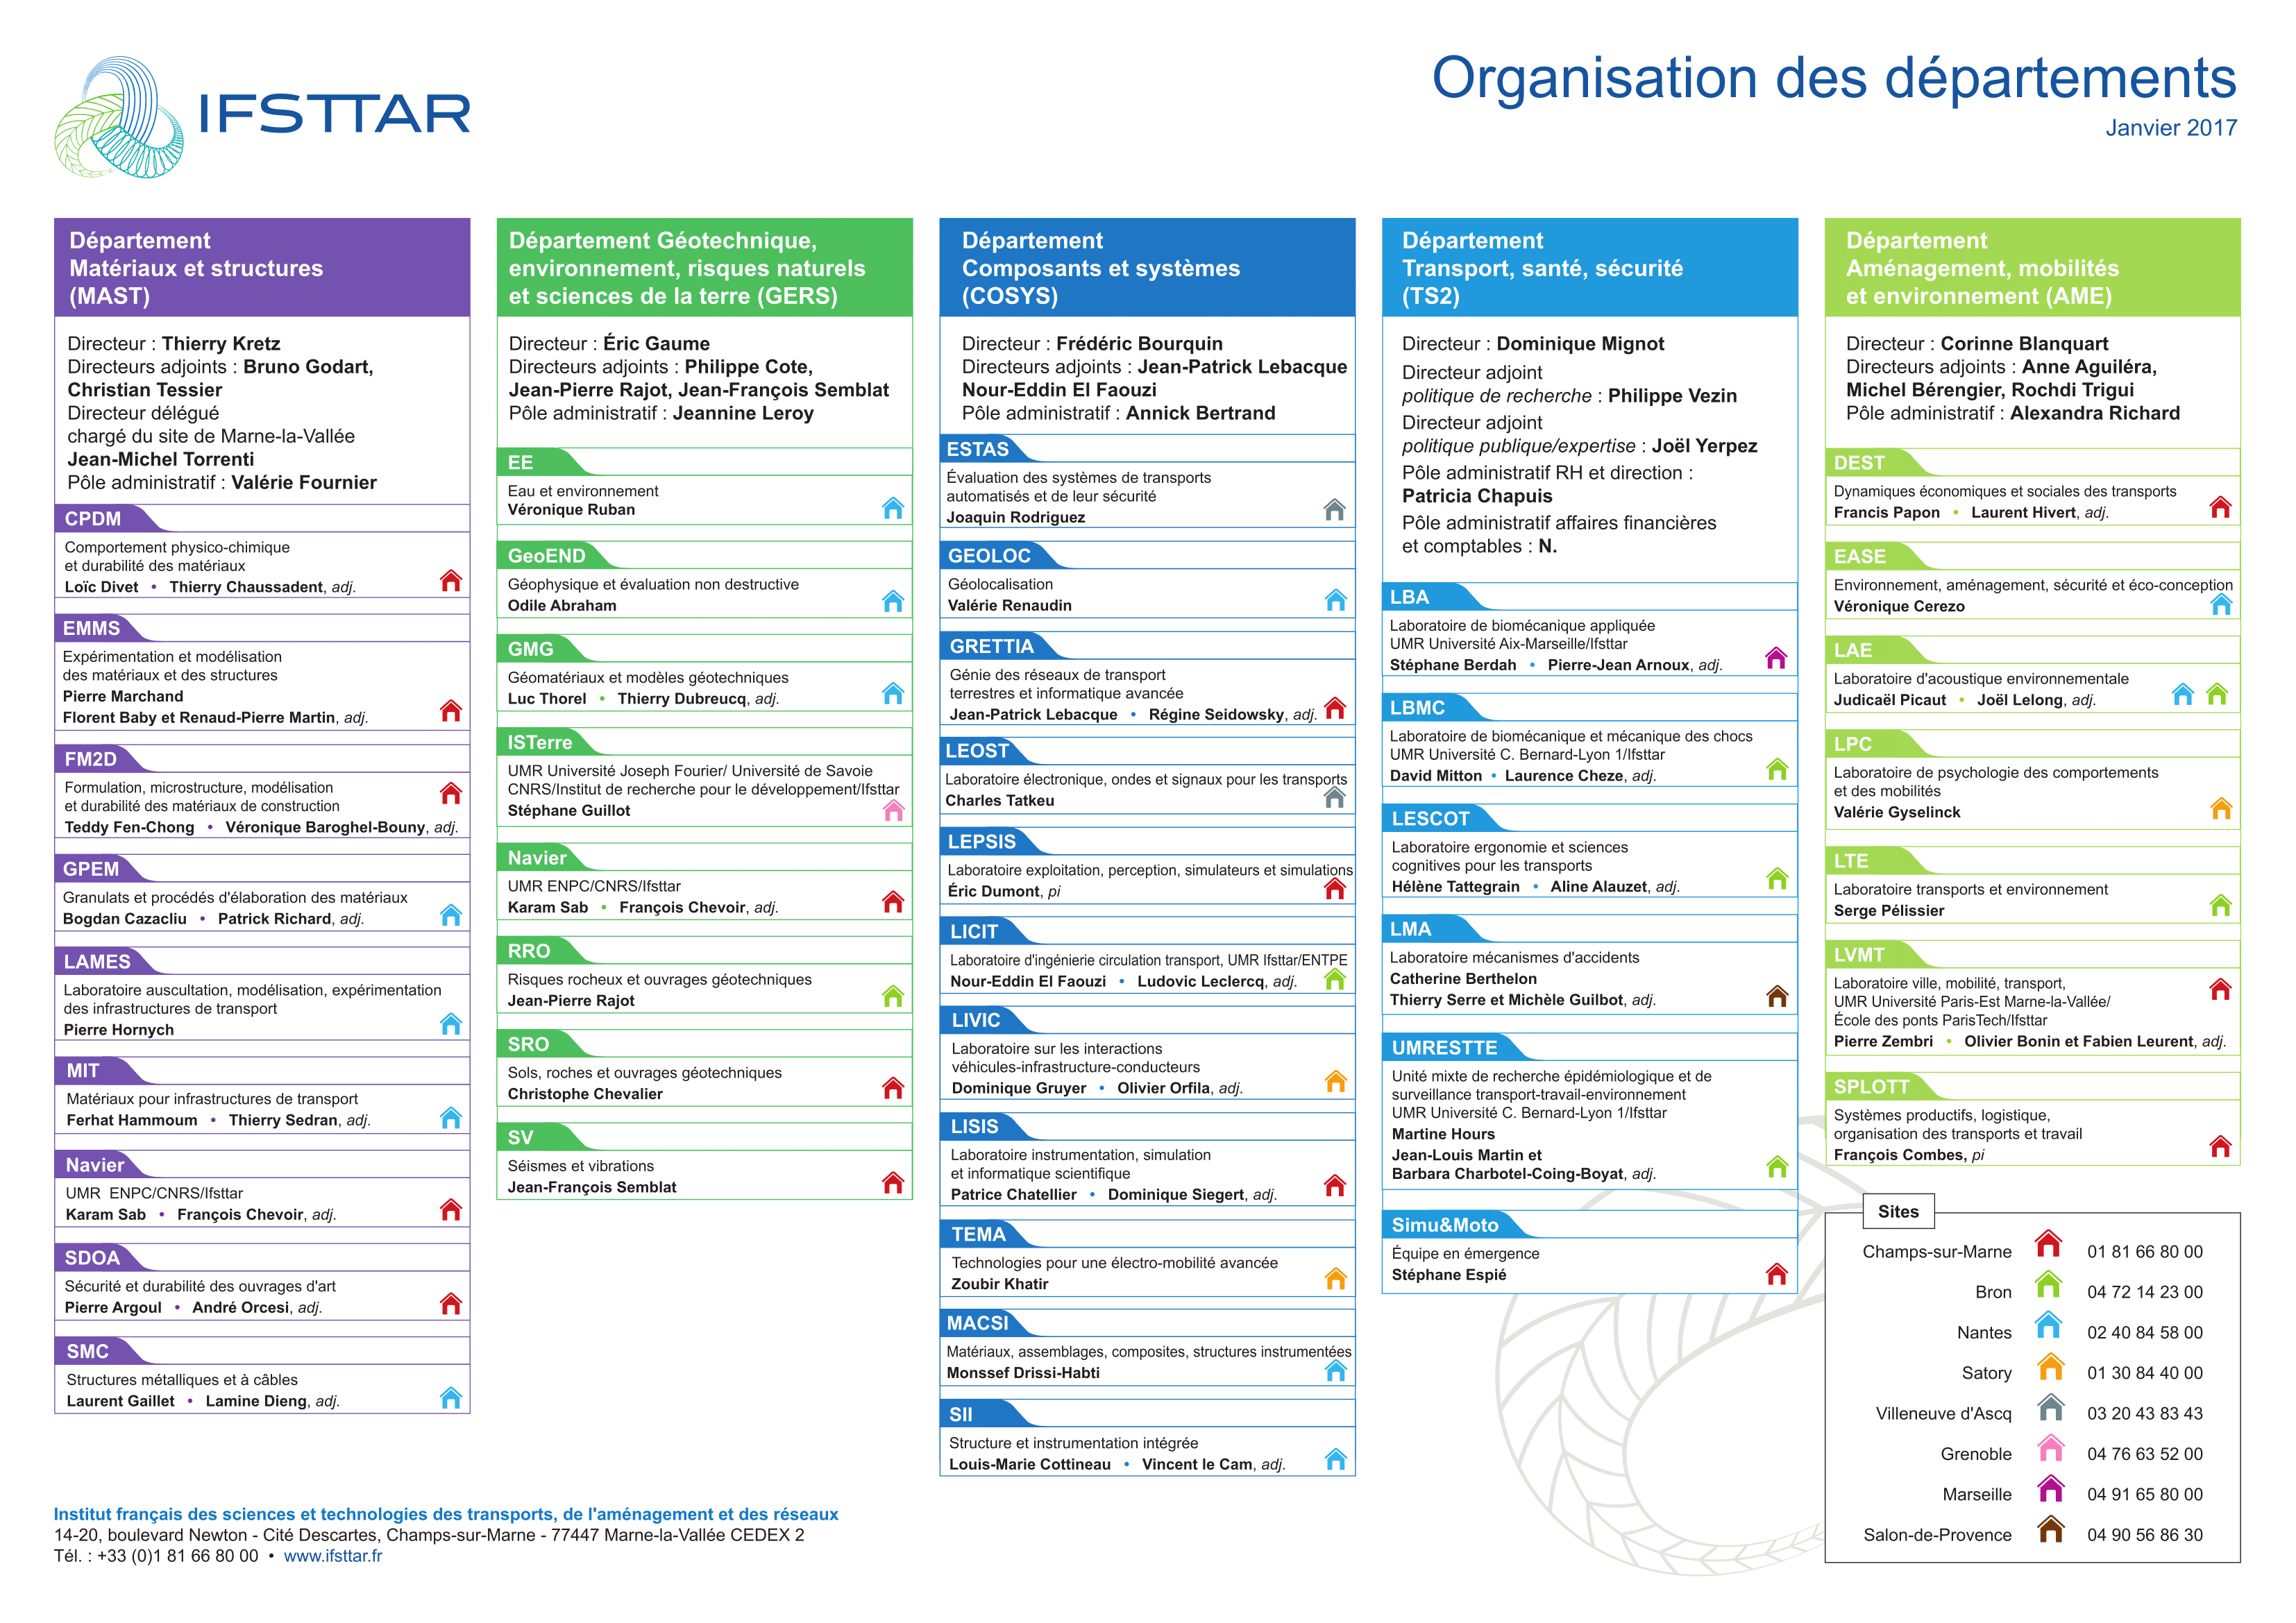
\includegraphics[width=\textwidth,height=\textheight,keepaspectratio]{annexes/organigramme_departements}

\addcontentsline{toc}{section}{B. Manuel utilisateur}
\includepdf[pages=1,offset=0 -3em,pagecommand={\section*{B. Manuel utilisateur}}]{\usermanualpath}
\includepdf[pages=2-]{\usermanualpath}

\documentclass[french,12pt]{article}



%%%%%%%%%%%%%%%%%%%%%%%%%%%%%%%%%%%%%%%%%%%%%%%%%%%%%%%%%%%%%%%%
%%%%%%%%%%%%%%%%%%%%%%%%%%%%%%%%%%%%%%%%%%%%%%%%%%%%%%%%%%%%%%%%
%%%%%%%%%%%%%%%%%%%%%%%%%%%%%%%%%%%%%%%%%%%%%%%%%%%%%%%%%%%%%%%%

\begin{document}


%%%%%%%%%%%%%%%%%%%%%%%%%%%%%%%%%%%%%%%%%%%%%%%%%%%%%%%%%%%%%%%%
%%%%%%%%%%%%%%%%%%%%%%%%%%%%%%%%%%%%%%%%%%%%%%%%%%%%%%%%%%%%%%%%
%%%%%%%%%%%%%%%%%%%%%%%%%%%%%%%%%%%%%%%%%%%%%%%%%%%%%%%%%%%%%%%%

\part{Présentation générale du problème}

\section{Projet}

\subsection{Finalité}

L'objectif de ce projet est de créer une base de données géo-référencées. Cette base est destinée à constituer un rassemblement volumineux de données géographiques sur le territoire. Les données sont rapatriées de sources diverses puis traitées automatiquement. Enfin, elle sont importées dans la base.

À des fins d'études recroisant ces données, cette base est vouée à être un source de données commune à de multiples utilisateurs. Dans cette optique, cette base sera munie d'un ensemble de requêtes basiques, c'est-à-dire de filtres larges permettant une utilisation facilitée de ces données par des logiciels de traitements, en aval.

\subsection{Problématique}

À l'\bsc{IFSTTAR}, certaines recherches requièrent la manipulation de données géographiques~: statistiques, recroisements, simulations. Actuellement le regroupement, stockage, filtrage, et partage de ces données est réalisé manuellement. Par conséquent, les mêmes manipulations sont souvent répétées, ce qui constitue une perte d'efforts et de temps.

\subsection{Énoncé du besoin}

Le travail à effectuer vise à créer un serveur de données centralisé en important automatiquement des données, en les pré-traitant, puis en les rapatriant dans la base.

L'utilisateur doit pouvoir définir l'ensembles paramètres d'exécution avant le lancement. Ainsi, sans modifier le code source, il doit être en mesure de spécifier les éléments énoncés ci-dessous.

\begin{description}
  \item[comportement~:] réaction du programme à une situation donnée (exemple~: niveau de verbosité)
  \item[structure de la base~:] tables, attributs, clés, relations, contraintes
  \item[données~:] source des données et traitements attendus (exemple~: spécifier la table qui va accueillir un ensemble de données)
\end{description}

L'ensemble de ces spécifications s'effectueront à travers des fichiers de configuration, de format \bsc{JSON}. Toute interaction entre le logiciel et l'utilisateur s'effectuera par ces fichiers. Ainsi, l'utilisateur n'aura pas besoin d'altérer le code source pour contrôler le comportement du logiciel.

De plus, seuls les paramètres absolument nécessaires seront à préciser, comme par exemple la structure de la base si l'utilisateur souhaite la créer. L'utilisateur aura bien entendu la liberté de redéfinir les autres paramètres au cas où leurs valeurs par défaut ne lui conviennent pas.

\subsection{Solution apportée}

Pour répondre au besoin énoncé ci-dessus, une base de données centralisée ainsi que des procédures d'importation, de nettoyage, et de traitement de données sont crées. L'ensemble de ces solutions permet notamment~:

\begin{itemize}
  \item un stockage massif performant de données
  \item l'élimination des tâches de pré-traitement~: récupération, nettoyage, uniformisation, recherche de liens (clés \& relations)
  \item la mutualisation des données, rendues accessibles à de multiples utilisateurs
  \item la mise à disposition de requêtes basiques de sélection avec application de filtres (attributaires, géographiques)
\end{itemize}

\subsection{Planification}

Diagramme de Gantt~:

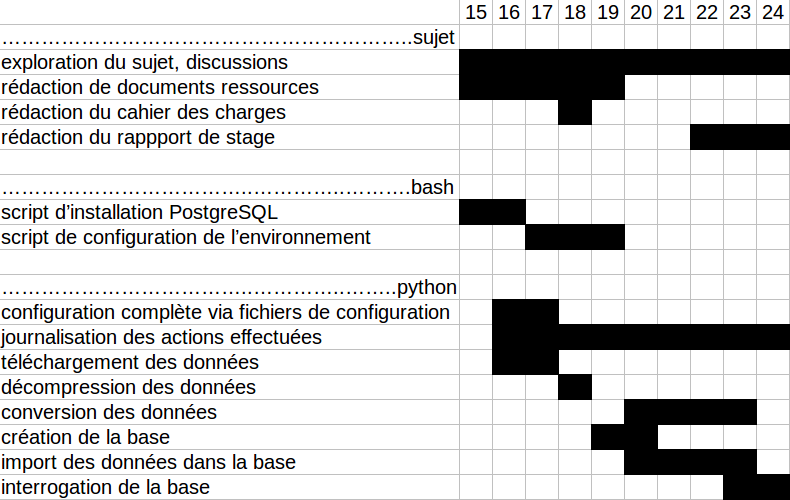
\includegraphics[height=25em]{gantt}

\section{Contexte}

\subsection{Études déjà effectuées}

Marc \bsc{Noël} a d'ores-et-déjà effectué un travail préliminaire sur les données et établi les liens existants. En effet, en parcourant et effectuant des traitements sur ces données il a pu conçevoir le schéma de la base de données.

C'est ce schéma qu'il revient ici d'implémenter, en discutant des adaptations mineures éventuelles. Ce schéma se veut proche des données d'entrée. De cette manière, l'intégration des données est facilitée.

\subsection{Nature des prestations demandées}

En premier lieu, le développement de deux scripts shell (\texttt{bash}). Ces scripts, non interactifs, vont venir préparer l'exécution ultérieure du code \texttt{Python}. En effet, ils se chargent de d'installer et configurer automatiquement l'ensemble des composants de l'environnement. Le premier se charge d'installer et de configurer la base \texttt{PostgreSQL}. Le second se charge de préparer l'exécution du code \texttt{Python} en installant les dépendances (les packages) auxquels il fait appel.

En second lieu, le développement d'un script \texttt{Python} chargé de manipuler les données. Ce dernier doit effectuer un ensemble de traitements tels que précisés par l'utilisateur.

\subsection{Parties concernées par le déroulement du projet et ses résultats}

En ce qui concerne l'\bsc{IUT} informatique de Nantes, Monsieur Loïg \bsc{Jezequel}, est chargé en tant qu'enseignant référent de suivre et évaluer ce stage. Ce suivi est réalisé via un message électronique envoyé en chaque fin de semaine, ainsi qu'une visite sur le lieu de stage. De même, plusieurs rendus sont à fournir tel qu'un résumé du sujet, ce cahier des charges, ainsi que le rapport de stage.

En ce qui concerne la structure d'accueil, l'\bsc{IFSTTAR}, Pascal \bsc{Gastineau} et Pierre \bsc{Hankach} jouent le rôle de tuteurs. Ils seront également les commanditaires et les clients du développement effectué.

Enfin, une soutenance ponctue le stage. Le jury sera alors composé de Pierre \bsc{Hankach}, Loïg \bsc{Jezequel}, ainsi qu'un second professeur de l'\bsc{IUT}.

\part{Détail technique du besoin}

\section{Étapes préliminaires~: scripts shell}

\subsection{Installation et configuration de \texttt{PostgreSQL}}

En premier lieu, le rôle de ce script est d'installer \texttt{PostgreSQL} et l'extension \texttt{PostGIS}.

En second lieu, ce script a pour rôle de configurer \texttt{PostgreSQL}. Cela est réalisé via l'édition automatisée de fichiers de configuration, et permet l'obtention des fonctionnalités suivantes~:

\begin{description}
  \item[compatibilité~:] support \bsc{UTF-8} pour la base \texttt{template1}
  \item[rôles~:] création de deux rôles (groupes) distincts permettant l'un la lecture et l'autre écriture ; ils seront hérités par les utilisateurs créés manuellement à posteriori
  \item[création~:] création de la base qui recevra les données
  \item[sécurité~:] ajout d'un mot de passe pour l'utilisateur \texttt{postgres}
  \item[journalisation~:] connexions et déconnexions
  \item[authentification] définition de la politique de sécurité
  \item[connexions~:] autorisation des connexions à distance
\end{description}

\subsection{Préparation de l'environnement d'exécution}

Le rôle de ce script est de préparer l'environnement d'exécution. Sa tâche principale est d'effectuer une installation de \texttt{miniconda} et d'importer un l'environnement adéquat. Cet environnement aura été préalablement exporté et conservé dans l'arborescence du projet.

\section{Applicatif \texttt{Python}}

\subsection{Description fonctionnelle}

Le code \texttt{Python} devra fournir les fonctionnalités suivantes~:

\begin{itemize}
  \item configuration complète via fichiers de configuration
  \item journalisation des actions effectuées
  \item téléchargement des données
  \item décompression des données
  \item conversion des données
  \item création de la base
  \item import des données dans la base
  \item interrogation de la base
\end{itemize}

\subsection{Modularité, découpage en sous-ensembles}

Le découpage en sous-ensembles s'articule autour de modules. Chaque module regroupe un ensemble logique de fonctionnalités. La figure suivante montre l'arbre décrivant une structure possible du projet.

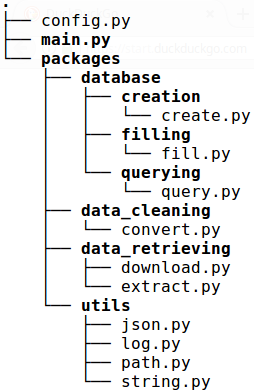
\includegraphics[height=15em]{arborescence}

Cette structure n'est pas définitive. En effet, elle est sujette à être étoffée ou redécoupée si nécessaire. Cependant, le découpage montrera toujours clairement les différentes tâches, de manière à les séparer. En effet les modules de plus haut niveau correspondent aux tâches principales de l'application.

%%%%%%%%%%%%%%%%%%%%%%%%%%%%%%%%%%%%%%%%%%%%%%%%%%%%%%%%%%%%%%%%
%%%%%%%%%%%%%%%%%%%%%%%%%%%%%%%%%%%%%%%%%%%%%%%%%%%%%%%%%%%%%%%%
%%%%%%%%%%%%%%%%%%%%%%%%%%%%%%%%%%%%%%%%%%%%%%%%%%%%%%%%%%%%%%%%

\end{document}

\section*{D. Journal de bord}
  \addcontentsline{toc}{section}{D. Journal de bord}

\paragraph{lundi 10/04/2017}
\begin{itemize}
  \item Visite du bâtiment
  \item Formalités administratives
  \item Installation environnement de travail (xfce, environnemment bash). Création mini-serveur samba pour échange facile de documents avec Marc
\end{itemize}

\paragraph{mardi 11/04/2017}
\begin{itemize}
  \item Collecte/lecture de tutoriels et documentation sur postgres
  \item Installation manuelle de postgres et premiers tests
\end{itemize}

\paragraph{mercredi 12/04/2017}
\begin{itemize}
  \item Réflexions sur les configurations post-installation à effectuer au sein du script
  \item Début d'un script bash de configuration de postgres
\end{itemize}

\paragraph{jeudi 13/04/2017}
\begin{itemize}
  \item Avancement sur le script et lecture doc postgres
\end{itemize}

\paragraph{vendredi 14/04/2017}
\begin{itemize}
  \item IFSTTAR fermé
\end{itemize}

\paragraph{lundi 17/04/2017}
\begin{itemize}
  \item IFSTTAR fermé
\end{itemize}

\paragraph{mardi 18/04/2017}
\begin{itemize}
  \item Petite réunion autour du script bash terminé. Questions/Réponses sur celui-ci et complétion de la documentation. Explication de mon script en détail
\end{itemize}

\paragraph{mercredi 19/04/2017}
\begin{itemize}
  \item Longue discussion avec Marc sur les intérêts de la création de cette base. Exemple "bureau de vote" sur des logiciels de traitement. Problématiques inhérentes aux traitements de données géo-référencées
  \item Rédaction d'un résumé du sujet de stage et de mes premières impressions
  \item Apprentissage du modèle de données créé par Marc
\end{itemize}

\paragraph{jeudi 20/04/2017}
\begin{itemize}
  \item Ajout d'une section "Troubleshooting" après la démarche d'installation qui donne des commandes bash utiles
  \item Python création de fonctions utilitaires de logs
\end{itemize}

\paragraph{vendredi 21/04/2017}
\begin{itemize}
  \item Passage de l'embryon de projet python sous PyCharm
  \item Lecture de PEPs
\end{itemize}

\paragraph{lundi 24/04/2017}
\begin{itemize}
  \item dev. début téléchargement
\end{itemize}

\paragraph{mardi 25/04/2017}
\begin{itemize}
  \item dev. téléchargement des archives
\end{itemize}

\paragraph{mercredi 26/04/2017}
\begin{itemize}
  \item Réflexions/discussions sur les interactions utilisateur
  \item Début de la création d'un "système de configuration"
\end{itemize}

\paragraph{jeudi 27/04/2017}
\begin{itemize}
  \item Système de configuration "intelligent" terminé
  \item Lecture de doc sur la librairie GDAL
\end{itemize}

\paragraph{vendredi 28/04/2017}
\begin{itemize}
  \item Nouveau script bash qui sépare la configuration de l'environnement pour python de celle puremment pour postgres
\end{itemize}

\paragraph{lundi 01/05/2017}
\begin{itemize}
  \item IFSTTAR fermé
\end{itemize}

\paragraph{mardi 02/05/2017}
\begin{itemize}
  \item Apprentissage de conda (miniconda sur dépôt conda-forge), environnements virtuels, pip
\end{itemize}

\paragraph{mercredi 03/05/2017}
\begin{itemize}
  \item Réunion : chacun présente son avancement
  \item Discussions sur ce qu'il y a à faire en priorité et sur les questions à creuser
  \item Décompression des archives téléchargées
\end{itemize}

\paragraph{jeudi 04/05/2017}
\begin{itemize}
  \item Lecture partielle du tutoriel SDZ/OC LaTeX
  \item Recherche et installation d'outils qui me conviennent pour éditer du LaTeX
  \item Squelette LaTeX cahier des charges
\end{itemize}

\paragraph{vendredi 05/05/2017}
\begin{itemize}
  \item Rédaction du cahier des charges
\end{itemize}

\paragraph{lundi 08/05/2017}
\begin{itemize}
  \item IFSTTAR fermé
\end{itemize}

\paragraph{mardi 09/05/2017}
\begin{itemize}
  \item Scripts bash pour conda terminés. 1 supplémentaire, standalone pour créer un venv et l'exporter
  \item Décompression via autodétection du type MIME
\end{itemize}

\paragraph{mercredi 10/05/2017}
\begin{itemize}
  \item Conception et réalisation : retours et réajustements sur le fichier de configuration des imports
\end{itemize}

\paragraph{jeudi 11/05/2017}
\begin{itemize}
  \item Renommage des archives téléchargées avec leur extension appropriée
  \item Tests et corrections mineures
\end{itemize}

\paragraph{vendredi 12/05/2017}
\begin{itemize}
  \item Modularisation en fonction des URI
  \item Conception algorithme de recherche pré-conversion
\end{itemize}

\paragraph{lundi 15/05/2017}
\begin{itemize}
  \item Implémentation de l'algorithme
  \item Tests
\end{itemize}

\paragraph{mardi 16/05/2017}
\begin{itemize}
  \item Finalisation de l'algorithme
  \item Discussions et décisions : entrée utilisateur (excel + script standalone de conversion)
  \item Retrait des modes automatiques dans le fichier de configuration des imports
\end{itemize}

\paragraph{mercredi 17/05/2017}
\begin{itemize}
  \item Distinguer les fichiers essentiels lors de la phase de tri/conversion
  \item Amélioration de la qualité des logs
\end{itemize}

\paragraph{jeudi 18/05/2017}
\begin{itemize}
  \item Lectures sur le mot-clé yield en python et les concepts rattachés
  \item Lecture sur les libraires (fiona, ogr2ogr) et sur les technos qui tournent autour
  \item Début parsage des données d'entrée avec Fiona
\end{itemize}

\paragraph{vendredi 19/05/2017}
\begin{itemize}
  \item 24h des IUT
\end{itemize}

\paragraph{lundi 22/05/2017}
\begin{itemize}
  \item Essais de modifications structurelles avec Fiona
\end{itemize}

\paragraph{mardi 23/05/2017}
\begin{itemize}
  \item Réunion discussion pour terminer la spécification du fonctionnement des fichiers de configuration
  \item Algorithme non testé de modifications structurelles des entrées en fonction des configurations
\end{itemize}

\paragraph{mercredi 24/05/2017}
\begin{itemize}
  \item Modifications structurelles selon config terminées et testées
  \item Clarification des logs
\end{itemize}

\paragraph{jeudi 25/05/2017}
\begin{itemize}
  \item IFSTTAR fermé
\end{itemize}

\paragraph{vendredi 26/05/2017}
\begin{itemize}
  \item IFSTTAR fermé
\end{itemize}

\paragraph{lundi 29/05/2017}
\begin{itemize}
  \item Conversion du excel vers fichier de configuration
\end{itemize}

\paragraph{mardi 30/05/2017}
\begin{itemize}
  \item Prise de connaissance du fonctionnement des schémas sous PostgreSQL
  \item Réalisation de la gestion automatique des schémas
\end{itemize}

\paragraph{mercredi 31/05/2017}
\begin{itemize}
  \item Résolution d'un problème avec les schémas
  \item Requêtes CREATE et INSERT fonctionnelles
\end{itemize}

\paragraph{jeudi 01/06/2017}
\begin{itemize}
  \item Tests et et listage/résolution des problèmes rencontrés
  \item Détermination des améliorations sur la structure, le nommage, et la documentation à effectuer
\end{itemize}

\paragraph{vendredi 02/06/2017}
\begin{itemize}
  \item Rédaction d'un manuel d'utilisation
\end{itemize}

\paragraph{lundi 05/06/2017}
\begin{itemize}
  \item IFSTTAR fermé
\end{itemize}

\paragraph{mardi 06/06/2017}
\begin{itemize}
  \item Début de patron LaTeX pour rapport
\end{itemize}

\paragraph{mercredi 07/06/2017}
\begin{itemize}
  \item Premier jet de structure sémantique du rapport
\end{itemize}

\paragraph{jeudi 08/06/2017}
\begin{itemize}
  \item Rédaction du rapport
\end{itemize}

\paragraph{vendredi 09/06/2017}
\begin{itemize}
  \item Rédaction du rapport
\end{itemize}

\paragraph{lundi 12/06/2017}
\begin{itemize}
  \item Rédaction du rapport
\end{itemize}

\paragraph{mardi 13/06/2017}
\begin{itemize}
  \item Rédaction du rapport
\end{itemize}

\paragraph{mercredi 14/06/2017}
\begin{itemize}
  \item Rédaction du rapport
\end{itemize}

\paragraph{jeudi 15/06/2017}
\begin{itemize}
  \item Relecture rapport et corrections mineures (numérotation, typos)
  \item Réalisation des diapositives pour la présentation
\end{itemize}

\paragraph{vendredi 15/06/2017}
\begin{itemize}
  \item Présentation du stage à l'\ifsttar
  \item Révision des diapositives
\end{itemize}

\paragraph{lundi 19/06/2017}
\begin{itemize}
  \item Soutenance de stage à l'\iut
  \item Listage des développements et améliorations à effectuer
\end{itemize}

\paragraph{mardi 20/06/2017}
\begin{itemize}
  \item Tests à partir des données finales à importer
  \item Ajout de la gestion du proxy pour la phase de téléchargement
\end{itemize}

\paragraph{mercredi 21/06/2017}
\begin{itemize}
  \item Continuation des tests
  \item Vérifications du comportement dans les cas marginaux
\end{itemize}

\paragraph{jeudi 22/06/2017}
\begin{itemize}
  \item Continuation des tests
  \item Vérifications du comportement dans les cas marginaux
\end{itemize}

\paragraph{vendredi 23/06/2017}
\begin{itemize}
  \item Petit point sur l'avancement du développement
  \item Passage de WKT en SRID
\end{itemize}

\clearpage



\end{document}
